%&program=xelatex
%&encoding=UTF-8 Unicode
% SVN keywords
% $Author$
% $Date$
% $Revision$
% $URL$
\documentclass[a4paper,twoside,12pt]{article}      % Comments after  % are ignored
%\usepackage{hyperref}                 % For creating hyperlinks in cross references
%\documentclass[a4paper,12pt]{article} 
%

\usepackage{ifxetex}% for XELATEX, or PDFlatex
\usepackage{ifplatform} 
%
\ifxetex
\usepackage{polyglossia} \setmainlanguage{portuges}
\usepackage{fontspec}
\ifwindows
\setmainfont[Ligatures=TeX]{Garamond}
\setsansfont[Ligatures=TeX]{Gill Sans MT}
	\setmonofont[Scale=0.95]{Courier}
	%\setmonofont[Scale=MatchLowercase]{Courier}	
\fi
\iflinux
\setmainfont[Ligatures=TeX]{Linux Libertine O}
\setsansfont[Ligatures=TeX,Scale=MatchLowercase]{Linux Biolinum}
\setmonofont[Scale=MatchLowercase]{Courier}
\fi
\ifmacosx
% add settings
\fi
%
\usepackage{xcolor,graphicx} 
\else
%PdfLaTEX
\usepackage[portuguese]{babel}
\usepackage[utf8]{inputenc}
\usepackage[T1]{fontenc}
\usepackage{graphics}                 % Packages to allow inclusion of graphics
\usepackage{color}                    % For creating coloured text and background
\fi

\usepackage{amsmath,amssymb,amsfonts} % Typical maths resource packages

\oddsidemargin 0cm
\evensidemargin 0cm

\pagestyle{myheadings}         % Option to put page headers
                               % Needed \documentclass[a4paper,twoside]{article}
\markboth{{\small\it MEFT - 2014/2015}}
{{\small\it Laboratório de Física Experimental Básica}}

\textwidth 15.5cm
\topmargin -1cm
\parindent 0cm
\textheight 24cm
\parskip 1mm


%\setmainfont[Ligatures=TeX]{Hoefler Text} 
%\setmainfont[Ligatures=TeX]{Times}
%\setsansfont[Ligatures=TeX,Scale=MatchLowercase]{Gill Sans} \setmonofont[Scale=MatchLowercase]{Courier}
%\setromanfont[Numbers=Uppercase]{Hoefler Text}
%\usepackage{xcolor,graphicx} 

%[pdftex]
%\usepackage{amsmath,amssymb} 
%\usepackage{amsmath} 
%\usepackage{textcomp}

% Math macros
\newcommand{\ud}{\,\mathrm{d}} 
\newcommand{\HRule}{\rule{\linewidth}{0.5mm}}

%\title{ e Difracção de Ondas Electromagnéticas num meio dieléctrico, homogéneo e isotrópico } 
%\subtitle{ aplicação à luz visível} 

\author{Prof. Bernardo B. Carvalho} 

%, Bernardo Brotas Carvalho\\bernardo@ipfn.ist.utl.pt} 
\date{ Setembro 2014} 

\begin{document} 

%	\begin{center}
%	\textsc{\large Laboratório de Física Experimental Básica - MEFT - 2012/2013 }\\%[0.5cm]
%	\end{center}

\includegraphics[width=0.2\textwidth]{../logo-ist}%\\[1cm]  %%  Logo_IST_color
	
	\HRule \\[0.5cm]
	{ \huge   \bfseries \textsc{ Pêndulo Gravítico } }\\[0.4cm]
	{ \large \bfseries Determinação do período do pêndulo simples e aferição com o valor da Aceleração da Gravidade local $g$  }\\
%	{ \large \begin{flushleft}
%	 $\bullet$ Deflexão magnética \\
%	 $\bullet$ Deflexão magnética em equilíbrio com deflexão eléctrica
%	\end{flushleft} }
	\HRule \\%[0.5cm]
%	\textsc{\Large Laboratório de Física Experimental Básica}\\[0.5cm]
	
%	\input{./title_exa.tex} 

%\maketitle
%\section{\sf  Conceitos necessários:} 
%\begin{enumerate}
%	\item Força eléctrica. Campo eléctrico (Electrostático)
%	\item Potencial eléctrico. Equipotencial. Energia potencial eléctrica 
%	\item Condutores e dieléctricos. Condensador plano
%	\item Efeitos da corrente eléctrica estacionária criada por uma espira 	
%	\item Força de Laplace
%\end{enumerate}

\section{\sf Movimento Harmónico Simples}

O Pêndulo Gravítico é um exemplo simples do modelo  matemático, o ``Oscilador Harmónico'' (OH), 
de essencial importância e  vastíssima utilização em quase todos o ramos da Física,
 bem como muitas áreas de Engenharia. 
 Neste modelo, um sistema físico arbitrário encontra-se na vizinhança de uma posição 
 de equilíbrio, onde há um mínimo local ou absoluto da sua Energia Potencial  ($E_P$). 
Ao distanciar-se deste mínimo, por uma perturbação ou outra qualquer força externa inicial, 
surge então uma força de índole conservativa, sempre direcionada de forma a repor o equilíbrio. 
Quando as forças exteriores deixam de actuar o sistema adquire movimento, 
transferindo-se a $E_P$ para Energia Cinética ($E_C$). 
Ao atingir a posição de equilíbrio e por inércia o movimento prossegue até se alcançar um 
novo máximo simétrico. 
Na ausência de forças dissipativas, o sistema regressa  ao ponto de partida e o ciclo repete-se infinitamente, com período $T_0$ constante (``Oscilador Livre''). Na presença de atrito a energia total deixa de ser constante e irá dissipar-se, diminuindo a amplitude do movimento, até desaparecer (``Oscilador Amortecido'').
% \begin{figure}
	% [t!bp]  \centering 
	% \includegraphics[width=0.45	\textwidth]{cucu} 
	% \caption{O Pêndulo gravítico foi até meados do sex. XX a forma mais exacta de medir o tempo. \label{fig:1}} 
% \end{figure}

%, no caso de Mecânica uma massa,
\subsection{\sf Sistema Massa-mola}
O exemplo de modelo OH mecânico mais simples  consiste num sistema de uma massa que se 
move na horizontal e sem atrito,  presa a uma mola  que é fixada na sua outra extremidade (Figura \ref{fig:2}). 
Caso a massa se deslocar da posição de equilíbrio ($x =0$), a Energia Potencial Elástica aumenta e mola irá exercer uma força de sinal contrário à deslocação, $\Delta x \equiv x - x_0 = x$.
 No modelo ideal da mola \emph{linear}  a força tem  módulo proporcional (com constante $k_{mola}$) ao deslocamento $x$ 

\begin{equation}
F_{mola} = - k_{mola} \, x \qquad 
\end{equation}

A partir da segunda equação de Newton, $F=m a$, e sabendo que $ a = \ddot{x}= \frac{d^2 x}{dt^2}$, é possível chegar facilmente  à equação de movimento do sistema Massa-Mola (equação diferencial de 2º grau)

\begin{equation}
	\label{eq:1} 
 m a = - k_{mola} x \Leftrightarrow \frac{d^2 x}{dt^2}  + \frac{k_{mola}}{m} x = 0
\end{equation}

%\Rightarrow
Pode-se verificar em poucos passos que a seguinte função temporal periódica é solução da equação (\ref{eq:1}).

\begin{equation}
	\label{eq:solu_mola}
x(t) = c_1 \cos(w_0 \, t) + c_2 \sin(w_0 \, t) = A_0 \sin(w_0 \, t + \phi_0) \text{, com } w_0 = \sqrt{\frac{k_{mola}}{m}}
\end{equation}

Com $ A_0 $ (Amplitude) e $\phi_0$ (fase) constantes, dependentes da condições iniciais. Finalmente $w_0$ é a frequência angular de ressonância que, inversa do período, depende apenas da massa, $m$ e de $k_{mola}$:
%, $\frac{2 \pi}{T}$,

\begin{equation}
	\label{eq:period_mola}
T_0 = \frac{2 \pi}{w_0} = 2\pi\; \sqrt{\frac{m}{k_{mola}}}	
\end{equation}

Assim, a solução para a posição, $x(t)$ ( e também para a velocidade \footnote{desfasada de $\pi/2$} $v(t)$), é uma função sinusoidal (harmónica).

\begin{figure}
	[!tbp] \centering 
	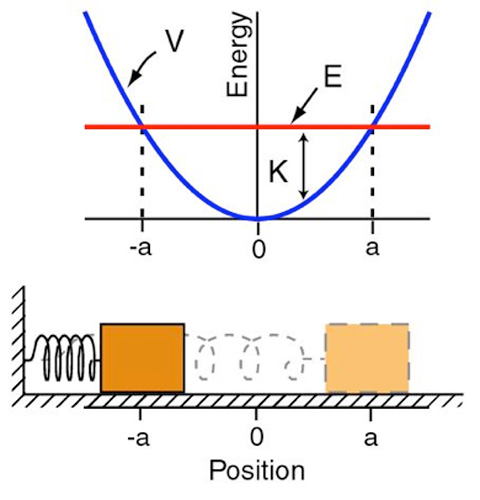
\includegraphics[width=0.5	\textwidth]{simple_harmonic_oscillator} 
	\caption{Oscilador Harmônico Simples \emph{Massa-Mola}.  \label{fig:2}} 
\end{figure}

\subsection{\sf Pêndulo gravítico}
O Pêndulo gravítico é também um sistema que pode ter como  modelo o ``Oscilador Harmónico'' e que consiste numa massa pontual suspensa\footnote{No Latim \emph{pendulus}} a partir de um fio virtualmente sem massa e comprimento $l$ fixo, que pode rodar em torno de um ponto (o ``pivôt"). Quando a massa se desvia da posição central, a força gravítica aplicada em $m$ (o peso $F_g = m \, g $) adquire uma componente na direcção de movimento (tangente à trajectória circular) e que tende a restabelecer o equilíbrio (Figura \ref{fig:3}). 

\begin{figure}
	[!htbp] \centering 
	
	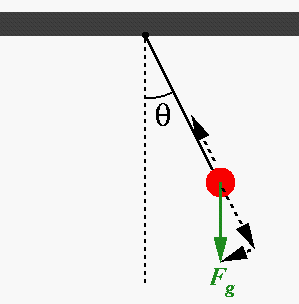
\includegraphics[width=0.5	\textwidth]{forcespend} \caption{Força de gravidade $F_g$ no pêndulo gravítico e a sua projeção na direção de movimento. \label{fig:3} } 
\end{figure}

Se o posição do pêndulo for descrita pela coordenada $s= l\cdot \theta$ ao longo da sua trajectória, 
então a força restauradora é 
\begin{equation}
	\label{eq:4} 
F_{tng} = - F_{g} \; sin(\theta) 
\end{equation}

E a equação diferencial de movimento 
\begin{align}
	\label{eq:5} 
	\frac{d^2 s}{dt^2} &=  l\;  \frac{d^2 \theta}{dt^2} \nonumber \\
	m \, l \, \frac{d^2 \theta}{dt^2} &= - m \,  g \, \sin(\theta)  \Rightarrow \frac{d^2 \theta}{dt^2} + \frac{g}{l} \sin(\theta) = 0
%l \,\frac{d^2 x}{dt^2} = \frac{k_{mola}}{m} x
\end{align}

Esta equação não tem uma resolução analítica simples, mas através do método  da \emph{linearização} (o ``canivete suíço'' dos Físicos), utiliza-se a aproximação $ \sin(\theta) \simeq \theta$ , para  $\theta_0 \le 0.08\,rad$ (aqui  os ângulos têm de ser medido em radianos!\footnote{ por exemplo: $\sin(5 ^{\circ}) = \sin(0.08726... \, \text{rad}) = 0.08715... $}).
Com esta aproximação ficamos com 

\begin{equation}
	\label{eq:6} 
	 \frac{d^2 \theta}{dt^2} + \frac{g}{l} \theta =0
\end{equation}

Cuja solução matemática é exacta e semelhante à expressão (\ref{eq:solu_mola})

\begin{equation}
	\label{eq:solu_pend}
\theta (t) = \theta_0 \sin(w_0 \, t + \phi_0) \text{, com } w_0 = \sqrt{\frac{g}{l}}
\end{equation}

O que é interessante neste modelo é que o efeito da \emph{massa gravítica } anula o da \emph{massa inercial } e o período do pêndulo fica a  depender apenas do comprimento $l$  e do valor da aceleração da Gravidade $g$  local 
\footnote{à superfície da Terra e à latitude de Lisboa: $g\approx 9.800\,m s^{-2}$. Consultar também o Projecto ``Pêndulo Mundial'', baseado no e-lab do IST: http://www.elab.ist.utl.pt/}
%à superfície da Terra $g\approx 9.81\,m s^{-2}$ e $g/\pi^2 \approx 0.994 \,m s^{-2}$}

\begin{equation}
	\label{eq:period_pend}
T_0 = \frac{2 \pi}{w_0} = 2\pi\; \sqrt{\frac{l}{g}} \text{, para }	\quad \theta_0 \ll 1
\end{equation}
%\simeq

Sabendo-se que já existiam pêndulos  desde a Antiguidade, foi o génio  Galileo Galilei, que no início do séc. XVII os estudou detalhadamente, chegando relação (\ref{eq:period_pend}).
A partir dessa altura
estes dispositivos foram sistemáticamente utilizados para medir o tempo, sendo a base 
de quase todos os relógios de precisão, com maior ou menor complexidades.
Actualmente apenas os relógios de Luxo usam uma variação do pêndulo, embora não seja gravitico.
(apenas a parte de geração energia, no relógios automático é gravítica. 
O único relógio ainda certificado para usar na Lua,
é um Omega de corda ... manual)

A resolução analítica (infelizmente bastante complexa) da equação 	(\ref{eq:5})  tem como solução para o período uma série  infinita de potências de $\theta_0$. 
Naturalmente, permite verificar que na aproximação $\theta_0 \ll 1$ a equação \ref{eq:period_pend} continua válida.
\begin{equation}
	\label{eq:period_pend_exa}
T_0 =  2\pi\, \sqrt{\frac{l}{g}} \left(1 + \frac{1}{16} \theta_0^{2} + \frac{11}{3072} \theta_0^{4} +
 \frac{737280}{3072} \theta_0^{6} + \frac{22931}{1321205760} \theta_0^{8} + \cdots \right)
\end{equation}

Até aqui desprezámos o atrito do ar no movimento do pêndulo. Ao introduzir esta contribuição, com a aproximação de atrito cinético 
proporcional à velocidade, a  equação	(\ref{eq:6}) muda para

\begin{equation}
%	\label{eq:6} 
	 \frac{d^2 \theta}{dt^2} + \lambda \, \frac{1}{m}  \frac{d \theta}{dt} + \frac{g}{l} \theta =0 \quad \lambda \text{ =Coeficiente de atrito viscoso}
\end{equation}

O primeiro efeito, que se pode verificar no laboratório é na amplitude do movimento $\theta_0$, que irá diminuir inexoravelmente com o tempo. 

O segundo efeito, muito mais difícil de observar, é que existe uma muito pequena alteração no período $T$
\begin{equation}
T_1= T_0 / \sqrt{1 - \zeta^2} 
\end{equation}

Com $ \zeta = \frac{\lambda}{2\, m} \sqrt{\frac{l}{g}}  $

O factor  $ \zeta $ também se pode relacionar com o factor de amortecimento $Q$ \footnote{Os Engenheiros chamam de factor de Qualidade} 
\begin{equation}
Q = 2 \pi \times \frac{\text{Energia do Pêndulo}}{\text{Energia perdida num ciclo}}
\end{equation}

\newpage
\section{\sf Procedimento Experimental}
{ \large Material }
 \begin{flushleft}
	 $\bullet$ Suporte do Pêndulo \\
	 $\bullet$ Massas de Chumbo, linha inextensível e com massa desprezável \\
	 $\bullet$ Régua graduada, Cronómetro, Fita métrica, transferidor, balança
\end{flushleft} 

Comece a sessão de laboratório por estimar a precisão que obtém na medição do tempo com o cronómetro, tendo em conta 
o tempo de reacção do corpo humano. 
Com a ajuda de um colega e de uma régua graduada obtenha 15 medidas da queda da régua e a partir da média e desvio padrão obtenha o seu tempo de reação e a incerteza \footnote{ $\,\overline{t}=\sqrt{\frac{2 \overline{D}}{g}}$ e   
$e_{\overline{t}}=\sqrt{\frac{2 }{g}} \cdot \frac{1}{2\sqrt{\overline{D}}} \cdot e_{\overline{D}}  
= \overline{t} \cdot \frac{1}{2\overline{D}} \cdot e_{\overline{D}} $ }

\begin{center}
\begin{tabular}{|r|c|c|c|}
\hline
Ensaio  & $D_A$ - Distância & $D_B$ - Distância & $D_C$ - Distância  \\
\# & de queda (cm) & de queda (cm) & de queda (cm)\\
\hline \hline
1 & & & \\
\hline
2 & &  &\\
\hline ... & & & \\
%\hline 4 & & & \\
\hline 15 & & & \\
\hline \hline
Média $\overline{D}$ (m) & &  & \\
Desvio padrão (m) & & & \\
Erro da Média  $e_{\overline{D}}$ (m) & & & \\ 
Tempo de reação $\overline{t} \pm e_{\overline{t}}$ (s) & $\qquad \pm$  & $\qquad \pm$  & $\qquad \pm$  \\
\hline
\end{tabular}
\end{center}

Monte o sistema de pêndulo gravítico e obtenha o período para diversos comprimentos do fio. 
Obtenha o valor de $g_{exp}$ para estes ensaios, usando a expressão (9), bem como a respectiva incerteza experimental. 
Compare o valor final de $g_{exp}$ obtido com o valor tabelado $g_{tab}$ e estime o desvio à exactidão que obteve. 

\smallskip

\subsection{\sf Aspectos a ter em conta:}

 \begin{flushleft}
	 $\bullet$ Uma massa pendurada num fio tem mais que o grau de liberdade em $\theta$. Tente assegurar-se que o pêndulo oscila apenas ao longo de um plano. \\
	 $\bullet$ Tente minimizar o efeitos de paralaxe na determinação dos ângulos\\
	 $\bullet$ Naturalmente a massa utilizada não é pontual. Quais os erros sistemático e aleatório na medida do comprimento $l$? \\	
	 $\bullet$ Como pode minimizar a incerteza da medição do período? Medindo o tempo num ou vários ciclos? \\
\end{flushleft} 

\subsection{\sf Actividades adicionais, se houver tempo:}

 \begin{flushleft}
	 $\bullet$ Verifique experimentalmente que o período do pêndulo não depende do valor da massa.\\
	 $\bullet$ Verifique experimentalmente que para grandes ângulos iniciais, o período do pêndulo varia. Aumenta ou diminue?\\
%	 Para que valores de $\theta_0$ o valor calculado de $g_{exp}$ se afasta de $\overline{g_{exp}}$ com desvio de $0.05$ ?\\
	 $\bullet$ Tente estimar a energia  devido ao atrito que se perde em cada ciclo (em percentagem).\\
	 $\bullet$ Qual o comprimento do pêndulo para construir um relógio pendular com período de $1\,s$? 
	 E se for na Lua?.
\end{flushleft} 

 
%\textbf{Ver descrição no guia de laboratório pgs.77-81}

\end{document} 	

